 \makeatletter \@ifundefined{rootpath}{% Manual to memoir http://mirrors.dotsrc.org/ctan/macros/latex/contrib/memoir/memman.pdf

%\documentclass[a4paper,12pt,fleqn,openany,twoside]{memoir} %two sides for printing
\documentclass[a4paper,12pt,fleqn,openany,oneside]{memoir} %one side for pdf
\usepackage[english]{babel}
\usepackage[utf8]{inputenc}
\usepackage{microtype}
\usepackage{paralist}

%Definitions
\usepackage{amsthm}
\theoremstyle{plain}
\newtheorem{thm}{Theorem}[chapter] % reset theorem numbering for each chapter
\theoremstyle{definition}
\newtheorem{defn}[thm]{Definition}


% Choses the depth of numerations
\setsecnumdepth{subsubsection}

% Choses the depth of toc
%\maxtocdepth{subsection}

% LaTeX logical statements
\usepackage{ifthen}

% Fancy space after use of e.g. command
\usepackage{xspace}

% Skips after paragraphs
\usepackage{parskip}

% Layout settings
\setlength{\parindent}{0cm}
\setlength{\parskip}{2ex plus 2ex} %kan udvides til f.eks: '2ex plus 2ex minus 0ex'

\sloppybottom

% Don't make a collection per default
\newcommand{\worksheetcollection}{false}

% Bibtex
\usepackage[square,numbers,sort,comma]{natbib}
%\usepackage{cite}
%\bibliographystyle{plainnat}
\bibliographystyle{IEEEtran}


% Fixmes
\usepackage{fixme}
\fxsetup{draft}

% Mathematic
\usepackage{amsmath}
\usepackage{amsfonts}
\usepackage{amssymb}
\usepackage{stmaryrd}
\allowdisplaybreaks[1]


% Acronyms
\usepackage[printonlyused]{acronym}

% Images
\usepackage{graphicx}
\usepackage{wrapfig}
\usepackage[outdir=./]{epstopdf}
\usepackage{epsfig}


% Captions ans subcaptions
\captionnamefont{\footnotesize\bfseries}
\captiontitlefont{\footnotesize}

% Enable memoir subfloats for figures and tables
\newsubfloat{figure}
\newsubfloat{table}

% Hack memoir subfigure styles to have bold label and footnotesize fonts
\renewcommand{\thesubfigure}{\footnotesize\bfseries{(\alph{subfigure})}}
\renewcommand{\thesubtable}{\footnotesize\bfseries{(\alph{subtable})}}

\renewcommand{\subcaption}[2][]{\subbottom[\footnotesize{#1}]{#2}}

% Memoir tweak pagenumbers
%\pagestyle{headings}

% Tikz
\usepackage{tikz}
\usetikzlibrary{arrows,shapes,calc,positioning}
\pgfmathsetseed{1}

%Pgf plots
\usepackage{pgfplots}
\pgfplotsset{compat=1.5}
% loatbarrier, keep figures within (sub,subsub) sections
\usepackage{placeins}
\usepackage{pgfplots}
\usepgfplotslibrary{units}
\usepackage[space-before-unit,range-units = repeat]{siunitx}

% Hyperlinked auto references
\usepackage[hidelinks]{hyperref}
\usepackage[nameinlink]{cleveref}
\crefname{lstlisting}{Listing}{Listings}  
\Crefname{lstlisting}{Listing}{Listings}

\crefname{thm}{definition}{definitions}
\Crefname{thm}{Definition}{Definitions}

%\def\chapterautorefname{Kapitel}
%\def\sectionautorefname{Afsnit}
%\def\subsectionautorefname{Afsnit}
%\def\subsubsectionautorefname{Underafsnit}
%\def\figureautorefname{Figur}
%\def\lstlistingautorefname{Listing}
%\def\lstnumberautorefname{Linje}
%\def\itemautorefname{Punkt}
\usepackage[hypcap]{caption} % Link to top of the figure and not the caption

%Sick shit to make \Autoref command
%http://tex.stackexchange.com/questions/36575/autorefs-inserted-text-has-not-the-correct-case
\def\HyLang@english{%
  \def\equationautorefname{Equation}%
  \def\footnoteautorefname{Footnote}%
  \def\itemautorefname{item}%
  \def\figureautorefname{Figure}%
  \def\tableautorefname{Table}%
  \def\partautorefname{Part}%
  \def\appendixautorefname{Appendix}%
  \def\chapterautorefname{Chapter}%
  \def\sectionautorefname{Section}%
  \def\subsectionautorefname{Subsection}%
  \def\subsubsectionautorefname{Subsubsection}%
  \def\paragraphautorefname{Paragraph}%
  \def\subparagraphautorefname{Subparagraph}%
  \def\FancyVerbLineautorefname{Line}%
  \def\theoremautorefname{Theorem}%
  \def\pageautorefname{Page}%
}

% Reference greencommentssections with number and name
\usepackage{nameref}
\newcommand{\bsnameref}[1]{\Cref{#1} ``\nameref{#1}''}
\newcommand{\bsref}[1]{\Cref{#1}}
\newcommand{\bsbilagref}[1]{Appendix \ref{#1}}
\newcommand{\bsbilagnameref}[1]{Appendix \ref{#1} ``\nameref{#1}''}
\newcommand{\pling}[1]{``#1''}


% Listings for code qoutes
\usepackage{listings}
%\usepackage[usenames,dvipsnames,svgnames,table]{xcolor}
\usepackage{color}
\usepackage{xcolor}
\definecolor{bluekeywords}{rgb}{0.13,0.13,1}
\definecolor{greencomments}{rgb}{0,0.5,0}
\definecolor{redstrings}{rgb}{0.9,0,0}
\usepackage{caption} 
\usepackage{multicol}
\DeclareCaptionFont{white}{\color{white}}
\DeclareCaptionFormat{listing}{\colorbox{gray}{\parbox{\textwidth}{#1#2#3}}}
\captionsetup[lstlisting]{format=listing,labelfont=white,textfont=white}
%\lstset{numbers=left}
\lstset{
	basicstyle=\footnotesize,
	tabsize=2,
	breaklines=true,
  literate={æ}{{\ae}}1 {ø}{{\o}}1 {å}{{\aa}}1 {Æ}{{\AE}}1 {Ø}{{\O}}1 {Å}{{\AA}}1,
  keywords={typeof, new, true, false, catch, function, return, null, catch, switch, var, if, in, while, do, else, case, break},
  keywordstyle=\color{blue}\bfseries,
  ndkeywords={class, export, boolean, throw, implements, import, this},
  ndkeywordstyle=\color{darkgray}\bfseries,
  identifierstyle=\color{black},
  sensitive=false,
  comment=[l]{//},
  morecomment=[s]{/*}{*/},
  commentstyle=\color{purple}\ttfamily,
  stringstyle=\color{red}\ttfamily,
  numbers=left,
  numbersep=-5pt,
  showstringspaces=false,
  showspaces=false,
  %morestring=[b]',
  %morestring=[b]"
}
\lstnewenvironment{code}[1][]%
  {\minipage{\linewidth} 
   \lstset{basicstyle=\ttfamily\footnotesize,frame=single,#1}}
  {\endminipage}

\lstdefinelanguage{scala}{
  morekeywords={abstract,case,catch,class,def,%
    do,else,extends,false,final,finally,%
    for,if,implicit,import,match,mixin,%
    new,null,object,override,package,%
    private,protected,requires,return,sealed,%
    super,this,throw,trait,true,try,%
    type,val,var,while,with,yield, Unit, Boolean, Int},
  otherkeywords={=>,<-,<\%,<:,>:,\#,@},
  sensitive=true,
  morecomment=[l]{//},
  morecomment=[n]{/*}{*/},
  morestring=[b]",
  morestring=[b]',
  morestring=[b]"""
}

\lstdefinelanguage{clojure}%
{morekeywords={*,*1,*2,*3,*agent*,*allow-unresolved-vars*,*assert*,*clojure-version*,*command-line-args*,%
*compile-files*,*compile-path*,*e,*err*,*file*,*flush-on-newline*,*in*,*macro-meta*,%
*math-context*,*ns*,*out*,*print-dup*,*print-length*,*print-level*,*print-meta*,*print-readably*,%
*read-eval*,*source-path*,*use-context-classloader*,*warn-on-reflection*,+,-,->,->>,..,/,:else,%
<,<=,=,==,>,>=,@,accessor,aclone,add-classpath,add-watch,agent,agent-errors,aget,alength,alias,%
all-ns,alter,alter-meta!,alter-var-root,amap,ancestors,and,apply,areduce,array-map,aset,%
aset-boolean,aset-byte,aset-char,aset-double,aset-float,aset-int,aset-long,aset-short,assert,%
assoc,assoc!,assoc-in,associative?,atom,await,await-for,await1,bases,bean,bigdec,bigint,binding,%
bit-and,bit-and-not,bit-clear,bit-flip,bit-not,bit-or,bit-set,bit-shift-left,bit-shift-right,%
bit-test,bit-xor,boolean,boolean-array,booleans,bound-fn,bound-fn*,butlast,byte,byte-array,%
bytes,cast,char,char-array,char-escape-string,char-name-string,char?,chars,chunk,chunk-append,%
chunk-buffer,chunk-cons,chunk-first,chunk-next,chunk-rest,chunked-seq?,class,class?,%
clear-agent-errors,clojure-version,coll?,comment,commute,comp,comparator,compare,compare-and-set!,%
compile,complement,concat,cond,condp,conj,conj!,cons,constantly,construct-proxy,contains?,count,%
counted?,create-ns,create-struct,cycle,dec,decimal?,declare,def,definline,defmacro,defmethod,%
defmulti,defn,defn-,defonce,defprotocol,defstruct,deftype,delay,delay?,deliver,deref,derive,%
descendants,destructure,disj,disj!,dissoc,dissoc!,distinct,distinct?,do,do-template,doall,doc,%
dorun,doseq,dosync,dotimes,doto,double,double-array,doubles,drop,drop-last,drop-while,empty,empty?,%
ensure,enumeration-seq,eval,even?,every?,false,false?,ffirst,file-seq,filter,finally,find,find-doc,%
find-ns,find-var,first,float,float-array,float?,floats,flush,fn,fn?,fnext,for,force,format,future,%
future-call,future-cancel,future-cancelled?,future-done?,future?,gen-class,gen-interface,gensym,%
get,get-in,get-method,get-proxy-class,get-thread-bindings,get-validator,hash,hash-map,hash-set,%
identical?,identity,if,if-let,if-not,ifn?,import,in-ns,inc,init-proxy,instance?,int,int-array,%
integer?,interleave,intern,interpose,into,into-array,ints,io!,isa?,iterate,iterator-seq,juxt,%
key,keys,keyword,keyword?,last,lazy-cat,lazy-seq,let,letfn,line-seq,list,list*,list?,load,load-file,%
load-reader,load-string,loaded-libs,locking,long,long-array,longs,loop,macroexpand,macroexpand-1,%
make-array,make-hierarchy,map,map?,mapcat,max,max-key,memfn,memoize,merge,merge-with,meta,%
method-sig,methods,min,min-key,mod,monitor-enter,monitor-exit,name,namespace,neg?,new,newline,%
next,nfirst,nil,nil?,nnext,not,not-any?,not-empty,not-every?,not=,ns,ns-aliases,ns-imports,%
ns-interns,ns-map,ns-name,ns-publics,ns-refers,ns-resolve,ns-unalias,ns-unmap,nth,nthnext,num,%
number?,odd?,or,parents,partial,partition,pcalls,peek,persistent!,pmap,pop,pop!,pop-thread-bindings,%
pos?,pr,pr-str,prefer-method,prefers,primitives-classnames,print,print-ctor,print-doc,print-dup,%
print-method,print-namespace-doc,print-simple,print-special-doc,print-str,printf,println,println-str,%
prn,prn-str,promise,proxy,proxy-call-with-super,proxy-mappings,proxy-name,proxy-super,%
push-thread-bindings,pvalues,quot,rand,rand-int,range,ratio?,rational?,rationalize,re-find,%
re-groups,re-matcher,re-matches,re-pattern,re-seq,read,read-line,read-string,recur,reduce,ref,%
ref-history-count,ref-max-history,ref-min-history,ref-set,refer,refer-clojure,reify,%
release-pending-sends,rem,remove,remove-method,remove-ns,remove-watch,repeat,repeatedly,%
replace,replicate,require,reset!,reset-meta!,resolve,rest,resultset-seq,reverse,reversible?,%
rseq,rsubseq,second,select-keys,send,send-off,seq,seq?,seque,sequence,sequential?,set,set!,%
set-validator!,set?,short,short-array,shorts,shutdown-agents,slurp,some,sort,sort-by,sorted-map,%
sorted-map-by,sorted-set,sorted-set-by,sorted?,special-form-anchor,special-symbol?,split-at,%
split-with,str,stream?,string?,struct,struct-map,subs,subseq,subvec,supers,swap!,symbol,symbol?,%
sync,syntax-symbol-anchor,take,take-last,take-nth,take-while,test,the-ns,throw,time,to-array,%
to-array-2d,trampoline,transient,tree-seq,true,true?,try,type,unchecked-add,unchecked-dec,%
unchecked-divide,unchecked-inc,unchecked-multiply,unchecked-negate,unchecked-remainder,%
unchecked-subtract,underive,unquote,unquote-splicing,update-in,update-proxy,use,val,vals,%
var,var-get,var-set,var?,vary-meta,vec,vector,vector?,when,when-first,when-let,when-not,%
while,with-bindings,with-bindings*,with-in-str,with-loading-context,with-local-vars,%
with-meta,with-open,with-out-str,with-precision,xml-seq,zero?,zipmap
},%
   sensitive,% ???
   alsodigit=-,%
   morecomment=[l];,%
   morestring=[b]"%
  }[keywords,comments,strings]%

% Worksheet commands
\newcommand{\worksheetstart}[5]{ %Title, Revision, Date, Author, rootpath
	\ifthenelse{\equal{\worksheetcollection}{false}}{
		\newcommand{\rootpath}{#5}
		\documentheader
		\chapter{#1}
	}{
		\chapter{#1}
	}
%	\vspace{-1em}
%	\textbf{\tiny Revision #2 at #3. Written by #4}\\
%	\textbf{\tiny Hovedansvarlig #4}\\
%	\vspace{2em}\\
}

\newcommand{\worksheetend}{
	\ifthenelse{\equal{\worksheetcollection}{false}}{
		\collectionend
	}{}
}

\newcommand{\documentheader}{
	% Draws a tikz camera
% #1 is the coordinate to the top left corner
% #2 is a label for the righthand center position
% #3 is the text shown in the center of the camera
\newcommand{\camera}[3]{
\coordinate (anchor) at #1;
\draw (anchor) -- ($ (anchor) + (0em,-20pt) $) -- ($ (anchor) + (10pt, -15pt) $) -- ($ (anchor) + (10pt,-5pt)$) -- cycle;
\draw ($ (anchor) + (10pt,-5pt) $) -- ($ (anchor) + (10pt,0pt) $) -- ($ (anchor) + (50pt,0pt) $) -- ($ (anchor) + (50pt,-20pt) $) -- node[yshift=10pt] {\tiny #3} ($ (anchor) + (10pt,-20pt) $)-- cycle;
\coordinate (#2) at ($ (anchor) + (50pt,-10pt) $);
}

\newcounter{frameNumber}
\newcommand{\frameWithSize}[3][false]{
	\stepcounter{frameNumber}
	\coordinate (anchor) at #2;
	\ifthenelse{\equal{#1}{false}}{
		\def\frameNumber{\arabic{frameNumber}}
	}{
		\def\frameNumber{#1}
	}
	\pgfmathtruncatemacro\randomnumber{random(0,4)}
	\node[yshift=20pt] at (anchor) {\frameNumber};
	\ifthenelse{\equal{#3}{I}}{
		\node[draw, minimum size=20pt, fill=green!60] at (anchor) {I};
		\filldraw[fill=gray] ($(anchor) + (-10pt,-40pt)$) rectangle ($(anchor) + (10pt,-20pt) + (0pt,\randomnumber pt)$);
	}{
		\ifthenelse{\equal{#3}{P}}{
			\node[draw, minimum size=20pt, fill=yellow!60] at (anchor) {P};
			\filldraw[fill=gray] ($(anchor) + (-10pt,-40pt)$) rectangle ($(anchor) + (10pt,-30pt) + (0pt,\randomnumber pt)$);
		}{
			\node[draw, minimum size=20pt, fill=blue!40!yellow!60!black] at (anchor) {\color{white}B};
			\filldraw[fill=gray] ($(anchor) + (-10pt,-40pt)$) rectangle ($(anchor) + (10pt,-37pt) + (0pt,\randomnumber pt)$);
		}
	}
	\draw[thick] ($(anchor) + (-10pt,-40pt)$) -- +(20pt,0pt);
}

	\begin{document}
	%\renewcommand{\chaptername}{Worksheet}
	\chapterstyle{section}
	\renewcommand{\beforechapskip}{0pt}
	\renewcommand{\afterchapskip}{0pt}
}

\newcommand{\collectionstart}[1]{
	\newcommand{\rootpath}{#1}
	\renewcommand{\worksheetcollection}{true}
	\documentheader
	\frontmatter
	%\forside
	\makeatletter \@ifundefined{rootpath}{% Manual to memoir http://mirrors.dotsrc.org/ctan/macros/latex/contrib/memoir/memman.pdf

%\documentclass[a4paper,12pt,fleqn,openany,twoside]{memoir} %two sides for printing
\documentclass[a4paper,12pt,fleqn,openany,oneside]{memoir} %one side for pdf
\usepackage[english]{babel}
\usepackage[utf8]{inputenc}
\usepackage{microtype}
\usepackage{paralist}

%Definitions
\usepackage{amsthm}
\theoremstyle{plain}
\newtheorem{thm}{Theorem}[chapter] % reset theorem numbering for each chapter
\theoremstyle{definition}
\newtheorem{defn}[thm]{Definition}


% Choses the depth of numerations
\setsecnumdepth{subsubsection}

% Choses the depth of toc
%\maxtocdepth{subsection}

% LaTeX logical statements
\usepackage{ifthen}

% Fancy space after use of e.g. command
\usepackage{xspace}

% Skips after paragraphs
\usepackage{parskip}

% Layout settings
\setlength{\parindent}{0cm}
\setlength{\parskip}{2ex plus 2ex} %kan udvides til f.eks: '2ex plus 2ex minus 0ex'

\sloppybottom

% Don't make a collection per default
\newcommand{\worksheetcollection}{false}

% Bibtex
\usepackage[square,numbers,sort,comma]{natbib}
%\usepackage{cite}
%\bibliographystyle{plainnat}
\bibliographystyle{IEEEtran}


% Fixmes
\usepackage{fixme}
\fxsetup{draft}

% Mathematic
\usepackage{amsmath}
\usepackage{amsfonts}
\usepackage{amssymb}
\usepackage{stmaryrd}
\allowdisplaybreaks[1]


% Acronyms
\usepackage[printonlyused]{acronym}

% Images
\usepackage{graphicx}
\usepackage{wrapfig}
\usepackage[outdir=./]{epstopdf}
\usepackage{epsfig}


% Captions ans subcaptions
\captionnamefont{\footnotesize\bfseries}
\captiontitlefont{\footnotesize}

% Enable memoir subfloats for figures and tables
\newsubfloat{figure}
\newsubfloat{table}

% Hack memoir subfigure styles to have bold label and footnotesize fonts
\renewcommand{\thesubfigure}{\footnotesize\bfseries{(\alph{subfigure})}}
\renewcommand{\thesubtable}{\footnotesize\bfseries{(\alph{subtable})}}

\renewcommand{\subcaption}[2][]{\subbottom[\footnotesize{#1}]{#2}}

% Memoir tweak pagenumbers
%\pagestyle{headings}

% Tikz
\usepackage{tikz}
\usetikzlibrary{arrows,shapes,calc,positioning}
\pgfmathsetseed{1}

%Pgf plots
\usepackage{pgfplots}
\pgfplotsset{compat=1.5}
% loatbarrier, keep figures within (sub,subsub) sections
\usepackage{placeins}
\usepackage{pgfplots}
\usepgfplotslibrary{units}
\usepackage[space-before-unit,range-units = repeat]{siunitx}

% Hyperlinked auto references
\usepackage[hidelinks]{hyperref}
\usepackage[nameinlink]{cleveref}
\crefname{lstlisting}{Listing}{Listings}  
\Crefname{lstlisting}{Listing}{Listings}

\crefname{thm}{definition}{definitions}
\Crefname{thm}{Definition}{Definitions}

%\def\chapterautorefname{Kapitel}
%\def\sectionautorefname{Afsnit}
%\def\subsectionautorefname{Afsnit}
%\def\subsubsectionautorefname{Underafsnit}
%\def\figureautorefname{Figur}
%\def\lstlistingautorefname{Listing}
%\def\lstnumberautorefname{Linje}
%\def\itemautorefname{Punkt}
\usepackage[hypcap]{caption} % Link to top of the figure and not the caption

%Sick shit to make \Autoref command
%http://tex.stackexchange.com/questions/36575/autorefs-inserted-text-has-not-the-correct-case
\def\HyLang@english{%
  \def\equationautorefname{Equation}%
  \def\footnoteautorefname{Footnote}%
  \def\itemautorefname{item}%
  \def\figureautorefname{Figure}%
  \def\tableautorefname{Table}%
  \def\partautorefname{Part}%
  \def\appendixautorefname{Appendix}%
  \def\chapterautorefname{Chapter}%
  \def\sectionautorefname{Section}%
  \def\subsectionautorefname{Subsection}%
  \def\subsubsectionautorefname{Subsubsection}%
  \def\paragraphautorefname{Paragraph}%
  \def\subparagraphautorefname{Subparagraph}%
  \def\FancyVerbLineautorefname{Line}%
  \def\theoremautorefname{Theorem}%
  \def\pageautorefname{Page}%
}

% Reference greencommentssections with number and name
\usepackage{nameref}
\newcommand{\bsnameref}[1]{\Cref{#1} ``\nameref{#1}''}
\newcommand{\bsref}[1]{\Cref{#1}}
\newcommand{\bsbilagref}[1]{Appendix \ref{#1}}
\newcommand{\bsbilagnameref}[1]{Appendix \ref{#1} ``\nameref{#1}''}
\newcommand{\pling}[1]{``#1''}


% Listings for code qoutes
\usepackage{listings}
%\usepackage[usenames,dvipsnames,svgnames,table]{xcolor}
\usepackage{color}
\usepackage{xcolor}
\definecolor{bluekeywords}{rgb}{0.13,0.13,1}
\definecolor{greencomments}{rgb}{0,0.5,0}
\definecolor{redstrings}{rgb}{0.9,0,0}
\usepackage{caption} 
\usepackage{multicol}
\DeclareCaptionFont{white}{\color{white}}
\DeclareCaptionFormat{listing}{\colorbox{gray}{\parbox{\textwidth}{#1#2#3}}}
\captionsetup[lstlisting]{format=listing,labelfont=white,textfont=white}
%\lstset{numbers=left}
\lstset{
	basicstyle=\footnotesize,
	tabsize=2,
	breaklines=true,
  literate={æ}{{\ae}}1 {ø}{{\o}}1 {å}{{\aa}}1 {Æ}{{\AE}}1 {Ø}{{\O}}1 {Å}{{\AA}}1,
  keywords={typeof, new, true, false, catch, function, return, null, catch, switch, var, if, in, while, do, else, case, break},
  keywordstyle=\color{blue}\bfseries,
  ndkeywords={class, export, boolean, throw, implements, import, this},
  ndkeywordstyle=\color{darkgray}\bfseries,
  identifierstyle=\color{black},
  sensitive=false,
  comment=[l]{//},
  morecomment=[s]{/*}{*/},
  commentstyle=\color{purple}\ttfamily,
  stringstyle=\color{red}\ttfamily,
  numbers=left,
  numbersep=-5pt,
  showstringspaces=false,
  showspaces=false,
  %morestring=[b]',
  %morestring=[b]"
}
\lstnewenvironment{code}[1][]%
  {\minipage{\linewidth} 
   \lstset{basicstyle=\ttfamily\footnotesize,frame=single,#1}}
  {\endminipage}

\lstdefinelanguage{scala}{
  morekeywords={abstract,case,catch,class,def,%
    do,else,extends,false,final,finally,%
    for,if,implicit,import,match,mixin,%
    new,null,object,override,package,%
    private,protected,requires,return,sealed,%
    super,this,throw,trait,true,try,%
    type,val,var,while,with,yield, Unit, Boolean, Int},
  otherkeywords={=>,<-,<\%,<:,>:,\#,@},
  sensitive=true,
  morecomment=[l]{//},
  morecomment=[n]{/*}{*/},
  morestring=[b]",
  morestring=[b]',
  morestring=[b]"""
}

\lstdefinelanguage{clojure}%
{morekeywords={*,*1,*2,*3,*agent*,*allow-unresolved-vars*,*assert*,*clojure-version*,*command-line-args*,%
*compile-files*,*compile-path*,*e,*err*,*file*,*flush-on-newline*,*in*,*macro-meta*,%
*math-context*,*ns*,*out*,*print-dup*,*print-length*,*print-level*,*print-meta*,*print-readably*,%
*read-eval*,*source-path*,*use-context-classloader*,*warn-on-reflection*,+,-,->,->>,..,/,:else,%
<,<=,=,==,>,>=,@,accessor,aclone,add-classpath,add-watch,agent,agent-errors,aget,alength,alias,%
all-ns,alter,alter-meta!,alter-var-root,amap,ancestors,and,apply,areduce,array-map,aset,%
aset-boolean,aset-byte,aset-char,aset-double,aset-float,aset-int,aset-long,aset-short,assert,%
assoc,assoc!,assoc-in,associative?,atom,await,await-for,await1,bases,bean,bigdec,bigint,binding,%
bit-and,bit-and-not,bit-clear,bit-flip,bit-not,bit-or,bit-set,bit-shift-left,bit-shift-right,%
bit-test,bit-xor,boolean,boolean-array,booleans,bound-fn,bound-fn*,butlast,byte,byte-array,%
bytes,cast,char,char-array,char-escape-string,char-name-string,char?,chars,chunk,chunk-append,%
chunk-buffer,chunk-cons,chunk-first,chunk-next,chunk-rest,chunked-seq?,class,class?,%
clear-agent-errors,clojure-version,coll?,comment,commute,comp,comparator,compare,compare-and-set!,%
compile,complement,concat,cond,condp,conj,conj!,cons,constantly,construct-proxy,contains?,count,%
counted?,create-ns,create-struct,cycle,dec,decimal?,declare,def,definline,defmacro,defmethod,%
defmulti,defn,defn-,defonce,defprotocol,defstruct,deftype,delay,delay?,deliver,deref,derive,%
descendants,destructure,disj,disj!,dissoc,dissoc!,distinct,distinct?,do,do-template,doall,doc,%
dorun,doseq,dosync,dotimes,doto,double,double-array,doubles,drop,drop-last,drop-while,empty,empty?,%
ensure,enumeration-seq,eval,even?,every?,false,false?,ffirst,file-seq,filter,finally,find,find-doc,%
find-ns,find-var,first,float,float-array,float?,floats,flush,fn,fn?,fnext,for,force,format,future,%
future-call,future-cancel,future-cancelled?,future-done?,future?,gen-class,gen-interface,gensym,%
get,get-in,get-method,get-proxy-class,get-thread-bindings,get-validator,hash,hash-map,hash-set,%
identical?,identity,if,if-let,if-not,ifn?,import,in-ns,inc,init-proxy,instance?,int,int-array,%
integer?,interleave,intern,interpose,into,into-array,ints,io!,isa?,iterate,iterator-seq,juxt,%
key,keys,keyword,keyword?,last,lazy-cat,lazy-seq,let,letfn,line-seq,list,list*,list?,load,load-file,%
load-reader,load-string,loaded-libs,locking,long,long-array,longs,loop,macroexpand,macroexpand-1,%
make-array,make-hierarchy,map,map?,mapcat,max,max-key,memfn,memoize,merge,merge-with,meta,%
method-sig,methods,min,min-key,mod,monitor-enter,monitor-exit,name,namespace,neg?,new,newline,%
next,nfirst,nil,nil?,nnext,not,not-any?,not-empty,not-every?,not=,ns,ns-aliases,ns-imports,%
ns-interns,ns-map,ns-name,ns-publics,ns-refers,ns-resolve,ns-unalias,ns-unmap,nth,nthnext,num,%
number?,odd?,or,parents,partial,partition,pcalls,peek,persistent!,pmap,pop,pop!,pop-thread-bindings,%
pos?,pr,pr-str,prefer-method,prefers,primitives-classnames,print,print-ctor,print-doc,print-dup,%
print-method,print-namespace-doc,print-simple,print-special-doc,print-str,printf,println,println-str,%
prn,prn-str,promise,proxy,proxy-call-with-super,proxy-mappings,proxy-name,proxy-super,%
push-thread-bindings,pvalues,quot,rand,rand-int,range,ratio?,rational?,rationalize,re-find,%
re-groups,re-matcher,re-matches,re-pattern,re-seq,read,read-line,read-string,recur,reduce,ref,%
ref-history-count,ref-max-history,ref-min-history,ref-set,refer,refer-clojure,reify,%
release-pending-sends,rem,remove,remove-method,remove-ns,remove-watch,repeat,repeatedly,%
replace,replicate,require,reset!,reset-meta!,resolve,rest,resultset-seq,reverse,reversible?,%
rseq,rsubseq,second,select-keys,send,send-off,seq,seq?,seque,sequence,sequential?,set,set!,%
set-validator!,set?,short,short-array,shorts,shutdown-agents,slurp,some,sort,sort-by,sorted-map,%
sorted-map-by,sorted-set,sorted-set-by,sorted?,special-form-anchor,special-symbol?,split-at,%
split-with,str,stream?,string?,struct,struct-map,subs,subseq,subvec,supers,swap!,symbol,symbol?,%
sync,syntax-symbol-anchor,take,take-last,take-nth,take-while,test,the-ns,throw,time,to-array,%
to-array-2d,trampoline,transient,tree-seq,true,true?,try,type,unchecked-add,unchecked-dec,%
unchecked-divide,unchecked-inc,unchecked-multiply,unchecked-negate,unchecked-remainder,%
unchecked-subtract,underive,unquote,unquote-splicing,update-in,update-proxy,use,val,vals,%
var,var-get,var-set,var?,vary-meta,vec,vector,vector?,when,when-first,when-let,when-not,%
while,with-bindings,with-bindings*,with-in-str,with-loading-context,with-local-vars,%
with-meta,with-open,with-out-str,with-precision,xml-seq,zero?,zipmap
},%
   sensitive,% ???
   alsodigit=-,%
   morecomment=[l];,%
   morestring=[b]"%
  }[keywords,comments,strings]%

% Worksheet commands
\newcommand{\worksheetstart}[5]{ %Title, Revision, Date, Author, rootpath
	\ifthenelse{\equal{\worksheetcollection}{false}}{
		\newcommand{\rootpath}{#5}
		\documentheader
		\chapter{#1}
	}{
		\chapter{#1}
	}
%	\vspace{-1em}
%	\textbf{\tiny Revision #2 at #3. Written by #4}\\
%	\textbf{\tiny Hovedansvarlig #4}\\
%	\vspace{2em}\\
}

\newcommand{\worksheetend}{
	\ifthenelse{\equal{\worksheetcollection}{false}}{
		\collectionend
	}{}
}

\newcommand{\documentheader}{
	\input{\rootpath/setup/tikz-commands.tex}
	\begin{document}
	%\renewcommand{\chaptername}{Worksheet}
	\chapterstyle{section}
	\renewcommand{\beforechapskip}{0pt}
	\renewcommand{\afterchapskip}{0pt}
}

\newcommand{\collectionstart}[1]{
	\newcommand{\rootpath}{#1}
	\renewcommand{\worksheetcollection}{true}
	\documentheader
	\frontmatter
	%\forside
	\input{\rootpath/worksheets/titlepage/titlepage}
	\input{\rootpath/worksheets/preface/preface}
	%\input{\rootpath/worksheets/forord/forord}
	\newpage
	\newpage
	\tableofcontents*
	\mainmatter
}

\newcommand{\collectionend}{
	\backmatter
	\chapter{List of Acronyms}\vspace{3em}
	\input{\rootpath/setup/acronyms}
	\bibliography{\rootpath/setup/bibliography}
	\end{document}
}


\newcommand{\bscode}{
	\lstinline
}

\newcommand{\bscodemath}[1]{
	\text{\lstinline|#1|}
}

\newcommand{\bsqoute}[2]{
	\begin{quote}
		\textit{``#1''}
		\begin{center}
			-- \emph{#2}
		\end{center}
	\end{quote}
}


\newcommand{\lag}{\langle}
\newcommand{\rag}{\rangle}
\newcommand{\besk}[1]{\ensuremath{\lag #1 \rag}}

\newcommand{\namedtodo}[5]
{
  \ifthenelse{\equal{#1}{}}
  {
    \todo[color=#4,caption=
    {\textbf{#3: } #2}]
    {\color{#5}\textbf{#3: }#2}
  }
  {
    \todo[color=#4,caption=
    {\textbf{#3: } #1}
    ,inline]
    {\color{#5}\textbf{#3: }#2}
  }
}
\newcommand{\andreas}[2][]{\namedtodo{#1}{#2}{Andreas}{blue!50!red!10}{black}}
\newcommand{\lone}[2][]{\namedtodo{#1}{#2}{Lone}{orange}{black}}
\definecolor{babypink}{rgb}{0.96, 0.76, 0.76}
\newcommand{\toby}[2][]{\namedtodo{#1}{#2}{Tobias}{babypink}{black}}
\newcommand{\kasper}[2][]{\namedtodo{#1}{#2}{Kasper}{green}{black}}

%multicol
\usepackage{multicol}

% todonotes
%\usepackage[disable]{todonotes} %For final report
\usepackage{todonotes} %For writing notes
\usepackage{fancyvrb}

%Loading AAU macro
\usepackage{lastpage}
%%%%%%%%%%%%%%%%%%%%%%%%%%%%%%%%%%%%%%%%%%%%%%%%
% Macros for the titlepage
%%%%%%%%%%%%%%%%%%%%%%%%%%%%%%%%%%%%%%%%%%%%%%%%
%Creates the aau titlepage
\newcommand{\aautitlepage}[3]{%
  {
    %set up various length
    \ifx\titlepageleftcolumnwidth\undefined
      \newlength{\titlepageleftcolumnwidth}
      \newlength{\titlepagerightcolumnwidth}
    \fi
    \setlength{\titlepageleftcolumnwidth}{0.5\textwidth-\tabcolsep}
    \setlength{\titlepagerightcolumnwidth}{\textwidth-2\tabcolsep-\titlepageleftcolumnwidth}
    %create title page
    \thispagestyle{empty}
    \noindent%
    \begin{tabular}{@{}ll@{}}
      \parbox{\titlepageleftcolumnwidth}{
        \iflanguage{danish}{%
          
\includegraphics[width=\titlepageleftcolumnwidth]{titlepage/figures/aau_logo_da}
        }{%
          
\includegraphics[width=\titlepageleftcolumnwidth]{titlepage/figures/aau_logo_en}
        }
      } &
      \parbox{\titlepagerightcolumnwidth}{\raggedleft\small
        #2
      }\bigskip\\
       #1 &
      \parbox[t]{\titlepagerightcolumnwidth}{%
      \textbf{Abstract:}\bigskip\par
        \fbox{\parbox{\titlepagerightcolumnwidth-2\fboxsep-2\fboxrule}{%
          #3
        }}
      }\\
    \end{tabular}
    \vfill  
    \clearpage
  }
}

% Environment for problem statements
% Can be auto referenced.
\newtheorem{problem}{Problem}
\def\problemautorefname{Problem}

%Create english project info
\newcommand{\englishprojectinfo}[6]{%
  \parbox[t]{\titlepageleftcolumnwidth}{
    \textbf{Title:}\\ #1\bigskip\par
    %\textbf{Theme:}\\ #2\bigskip\par
    \textbf{Project Period:}\\ #2\bigskip\par
    \textbf{Project Group:}\\ #3\bigskip\par
    \textbf{Participants:}\\ #4\bigskip\par
    \textbf{Supervisor:}\\ #5\bigskip\par
    %\textbf{Copies:} #6\bigskip\par
    \textbf{Page Numbers:} \pageref{LastPage}\bigskip\par
    \textbf{Date of Completion:}\\ #6
  }
}



%Create danish project info
%\newcommand{\danishprojectinfo}[7]{%
 % \parbox[t]{\titlepageleftcolumnwidth}{
 %   \textbf{Titel:}\\ #1\bigskip\par
%    %\textbf{Tema:}\\ #2\bigskip\par
%    \textbf{Projektperiode:}\\ #2\bigskip\par
%    \textbf{Projektgruppe:}\\ #4\bigskip\par
%    \textbf{Deltager(e):}\\ #5\bigskip\par
 %   \textbf{Vejleder(e):}\\ #6\bigskip\par
%    \textbf{Oplagstal:} #7\bigskip\par
   % \textbf{Sidetal:} \pageref{LastPage}\bigskip\par
  %  \textbf{Afleveringsdato:}\\ #8
 % }
%}
}\makeatother
%\worksheetstart{Titlepage}{0}{December 31, 2012}{../../}
\begin{titlingpage}
\aautitlepage{%
  \englishprojectinfo{
    Scalable webservices %title
  }{%
    Spring Semester 2014 %project period
  }{%
    it801f14  % project group
  }{%
    %list of group members
    Tobias Ugleholdt Hansen\\
    Andreas Pørtner Karlsen\\ 
    Kasper Breinholt Laurberg\\
  }{%
    %list of supervisors
     Lone 
  }{%
    \today % date of completion
  }%
}{%department and address
  \textbf{Department of Computer Science}\\
  Selma Lagerløfs Vej 300\\
  DK-9220 Aalborg Ø\\
  \href{http://www.cs.aau.dk}{http://www.cs.aau.dk}
}{% the abstract
Some nice abstract
}
\end{titlingpage}
	\makeatletter \@ifundefined{rootpath}{% Manual to memoir http://mirrors.dotsrc.org/ctan/macros/latex/contrib/memoir/memman.pdf

%\documentclass[a4paper,12pt,fleqn,openany,twoside]{memoir} %two sides for printing
\documentclass[a4paper,12pt,fleqn,openany,oneside]{memoir} %one side for pdf
\usepackage[english]{babel}
\usepackage[utf8]{inputenc}
\usepackage{microtype}
\usepackage{paralist}

%Definitions
\usepackage{amsthm}
\theoremstyle{plain}
\newtheorem{thm}{Theorem}[chapter] % reset theorem numbering for each chapter
\theoremstyle{definition}
\newtheorem{defn}[thm]{Definition}


% Choses the depth of numerations
\setsecnumdepth{subsubsection}

% Choses the depth of toc
%\maxtocdepth{subsection}

% LaTeX logical statements
\usepackage{ifthen}

% Fancy space after use of e.g. command
\usepackage{xspace}

% Skips after paragraphs
\usepackage{parskip}

% Layout settings
\setlength{\parindent}{0cm}
\setlength{\parskip}{2ex plus 2ex} %kan udvides til f.eks: '2ex plus 2ex minus 0ex'

\sloppybottom

% Don't make a collection per default
\newcommand{\worksheetcollection}{false}

% Bibtex
\usepackage[square,numbers,sort,comma]{natbib}
%\usepackage{cite}
%\bibliographystyle{plainnat}
\bibliographystyle{IEEEtran}


% Fixmes
\usepackage{fixme}
\fxsetup{draft}

% Mathematic
\usepackage{amsmath}
\usepackage{amsfonts}
\usepackage{amssymb}
\usepackage{stmaryrd}
\allowdisplaybreaks[1]


% Acronyms
\usepackage[printonlyused]{acronym}

% Images
\usepackage{graphicx}
\usepackage{wrapfig}
\usepackage[outdir=./]{epstopdf}
\usepackage{epsfig}


% Captions ans subcaptions
\captionnamefont{\footnotesize\bfseries}
\captiontitlefont{\footnotesize}

% Enable memoir subfloats for figures and tables
\newsubfloat{figure}
\newsubfloat{table}

% Hack memoir subfigure styles to have bold label and footnotesize fonts
\renewcommand{\thesubfigure}{\footnotesize\bfseries{(\alph{subfigure})}}
\renewcommand{\thesubtable}{\footnotesize\bfseries{(\alph{subtable})}}

\renewcommand{\subcaption}[2][]{\subbottom[\footnotesize{#1}]{#2}}

% Memoir tweak pagenumbers
%\pagestyle{headings}

% Tikz
\usepackage{tikz}
\usetikzlibrary{arrows,shapes,calc,positioning}
\pgfmathsetseed{1}

%Pgf plots
\usepackage{pgfplots}
\pgfplotsset{compat=1.5}
% loatbarrier, keep figures within (sub,subsub) sections
\usepackage{placeins}
\usepackage{pgfplots}
\usepgfplotslibrary{units}
\usepackage[space-before-unit,range-units = repeat]{siunitx}

% Hyperlinked auto references
\usepackage[hidelinks]{hyperref}
\usepackage[nameinlink]{cleveref}
\crefname{lstlisting}{Listing}{Listings}  
\Crefname{lstlisting}{Listing}{Listings}

\crefname{thm}{definition}{definitions}
\Crefname{thm}{Definition}{Definitions}

%\def\chapterautorefname{Kapitel}
%\def\sectionautorefname{Afsnit}
%\def\subsectionautorefname{Afsnit}
%\def\subsubsectionautorefname{Underafsnit}
%\def\figureautorefname{Figur}
%\def\lstlistingautorefname{Listing}
%\def\lstnumberautorefname{Linje}
%\def\itemautorefname{Punkt}
\usepackage[hypcap]{caption} % Link to top of the figure and not the caption

%Sick shit to make \Autoref command
%http://tex.stackexchange.com/questions/36575/autorefs-inserted-text-has-not-the-correct-case
\def\HyLang@english{%
  \def\equationautorefname{Equation}%
  \def\footnoteautorefname{Footnote}%
  \def\itemautorefname{item}%
  \def\figureautorefname{Figure}%
  \def\tableautorefname{Table}%
  \def\partautorefname{Part}%
  \def\appendixautorefname{Appendix}%
  \def\chapterautorefname{Chapter}%
  \def\sectionautorefname{Section}%
  \def\subsectionautorefname{Subsection}%
  \def\subsubsectionautorefname{Subsubsection}%
  \def\paragraphautorefname{Paragraph}%
  \def\subparagraphautorefname{Subparagraph}%
  \def\FancyVerbLineautorefname{Line}%
  \def\theoremautorefname{Theorem}%
  \def\pageautorefname{Page}%
}

% Reference greencommentssections with number and name
\usepackage{nameref}
\newcommand{\bsnameref}[1]{\Cref{#1} ``\nameref{#1}''}
\newcommand{\bsref}[1]{\Cref{#1}}
\newcommand{\bsbilagref}[1]{Appendix \ref{#1}}
\newcommand{\bsbilagnameref}[1]{Appendix \ref{#1} ``\nameref{#1}''}
\newcommand{\pling}[1]{``#1''}


% Listings for code qoutes
\usepackage{listings}
%\usepackage[usenames,dvipsnames,svgnames,table]{xcolor}
\usepackage{color}
\usepackage{xcolor}
\definecolor{bluekeywords}{rgb}{0.13,0.13,1}
\definecolor{greencomments}{rgb}{0,0.5,0}
\definecolor{redstrings}{rgb}{0.9,0,0}
\usepackage{caption} 
\usepackage{multicol}
\DeclareCaptionFont{white}{\color{white}}
\DeclareCaptionFormat{listing}{\colorbox{gray}{\parbox{\textwidth}{#1#2#3}}}
\captionsetup[lstlisting]{format=listing,labelfont=white,textfont=white}
%\lstset{numbers=left}
\lstset{
	basicstyle=\footnotesize,
	tabsize=2,
	breaklines=true,
  literate={æ}{{\ae}}1 {ø}{{\o}}1 {å}{{\aa}}1 {Æ}{{\AE}}1 {Ø}{{\O}}1 {Å}{{\AA}}1,
  keywords={typeof, new, true, false, catch, function, return, null, catch, switch, var, if, in, while, do, else, case, break},
  keywordstyle=\color{blue}\bfseries,
  ndkeywords={class, export, boolean, throw, implements, import, this},
  ndkeywordstyle=\color{darkgray}\bfseries,
  identifierstyle=\color{black},
  sensitive=false,
  comment=[l]{//},
  morecomment=[s]{/*}{*/},
  commentstyle=\color{purple}\ttfamily,
  stringstyle=\color{red}\ttfamily,
  numbers=left,
  numbersep=-5pt,
  showstringspaces=false,
  showspaces=false,
  %morestring=[b]',
  %morestring=[b]"
}
\lstnewenvironment{code}[1][]%
  {\minipage{\linewidth} 
   \lstset{basicstyle=\ttfamily\footnotesize,frame=single,#1}}
  {\endminipage}

\lstdefinelanguage{scala}{
  morekeywords={abstract,case,catch,class,def,%
    do,else,extends,false,final,finally,%
    for,if,implicit,import,match,mixin,%
    new,null,object,override,package,%
    private,protected,requires,return,sealed,%
    super,this,throw,trait,true,try,%
    type,val,var,while,with,yield, Unit, Boolean, Int},
  otherkeywords={=>,<-,<\%,<:,>:,\#,@},
  sensitive=true,
  morecomment=[l]{//},
  morecomment=[n]{/*}{*/},
  morestring=[b]",
  morestring=[b]',
  morestring=[b]"""
}

\lstdefinelanguage{clojure}%
{morekeywords={*,*1,*2,*3,*agent*,*allow-unresolved-vars*,*assert*,*clojure-version*,*command-line-args*,%
*compile-files*,*compile-path*,*e,*err*,*file*,*flush-on-newline*,*in*,*macro-meta*,%
*math-context*,*ns*,*out*,*print-dup*,*print-length*,*print-level*,*print-meta*,*print-readably*,%
*read-eval*,*source-path*,*use-context-classloader*,*warn-on-reflection*,+,-,->,->>,..,/,:else,%
<,<=,=,==,>,>=,@,accessor,aclone,add-classpath,add-watch,agent,agent-errors,aget,alength,alias,%
all-ns,alter,alter-meta!,alter-var-root,amap,ancestors,and,apply,areduce,array-map,aset,%
aset-boolean,aset-byte,aset-char,aset-double,aset-float,aset-int,aset-long,aset-short,assert,%
assoc,assoc!,assoc-in,associative?,atom,await,await-for,await1,bases,bean,bigdec,bigint,binding,%
bit-and,bit-and-not,bit-clear,bit-flip,bit-not,bit-or,bit-set,bit-shift-left,bit-shift-right,%
bit-test,bit-xor,boolean,boolean-array,booleans,bound-fn,bound-fn*,butlast,byte,byte-array,%
bytes,cast,char,char-array,char-escape-string,char-name-string,char?,chars,chunk,chunk-append,%
chunk-buffer,chunk-cons,chunk-first,chunk-next,chunk-rest,chunked-seq?,class,class?,%
clear-agent-errors,clojure-version,coll?,comment,commute,comp,comparator,compare,compare-and-set!,%
compile,complement,concat,cond,condp,conj,conj!,cons,constantly,construct-proxy,contains?,count,%
counted?,create-ns,create-struct,cycle,dec,decimal?,declare,def,definline,defmacro,defmethod,%
defmulti,defn,defn-,defonce,defprotocol,defstruct,deftype,delay,delay?,deliver,deref,derive,%
descendants,destructure,disj,disj!,dissoc,dissoc!,distinct,distinct?,do,do-template,doall,doc,%
dorun,doseq,dosync,dotimes,doto,double,double-array,doubles,drop,drop-last,drop-while,empty,empty?,%
ensure,enumeration-seq,eval,even?,every?,false,false?,ffirst,file-seq,filter,finally,find,find-doc,%
find-ns,find-var,first,float,float-array,float?,floats,flush,fn,fn?,fnext,for,force,format,future,%
future-call,future-cancel,future-cancelled?,future-done?,future?,gen-class,gen-interface,gensym,%
get,get-in,get-method,get-proxy-class,get-thread-bindings,get-validator,hash,hash-map,hash-set,%
identical?,identity,if,if-let,if-not,ifn?,import,in-ns,inc,init-proxy,instance?,int,int-array,%
integer?,interleave,intern,interpose,into,into-array,ints,io!,isa?,iterate,iterator-seq,juxt,%
key,keys,keyword,keyword?,last,lazy-cat,lazy-seq,let,letfn,line-seq,list,list*,list?,load,load-file,%
load-reader,load-string,loaded-libs,locking,long,long-array,longs,loop,macroexpand,macroexpand-1,%
make-array,make-hierarchy,map,map?,mapcat,max,max-key,memfn,memoize,merge,merge-with,meta,%
method-sig,methods,min,min-key,mod,monitor-enter,monitor-exit,name,namespace,neg?,new,newline,%
next,nfirst,nil,nil?,nnext,not,not-any?,not-empty,not-every?,not=,ns,ns-aliases,ns-imports,%
ns-interns,ns-map,ns-name,ns-publics,ns-refers,ns-resolve,ns-unalias,ns-unmap,nth,nthnext,num,%
number?,odd?,or,parents,partial,partition,pcalls,peek,persistent!,pmap,pop,pop!,pop-thread-bindings,%
pos?,pr,pr-str,prefer-method,prefers,primitives-classnames,print,print-ctor,print-doc,print-dup,%
print-method,print-namespace-doc,print-simple,print-special-doc,print-str,printf,println,println-str,%
prn,prn-str,promise,proxy,proxy-call-with-super,proxy-mappings,proxy-name,proxy-super,%
push-thread-bindings,pvalues,quot,rand,rand-int,range,ratio?,rational?,rationalize,re-find,%
re-groups,re-matcher,re-matches,re-pattern,re-seq,read,read-line,read-string,recur,reduce,ref,%
ref-history-count,ref-max-history,ref-min-history,ref-set,refer,refer-clojure,reify,%
release-pending-sends,rem,remove,remove-method,remove-ns,remove-watch,repeat,repeatedly,%
replace,replicate,require,reset!,reset-meta!,resolve,rest,resultset-seq,reverse,reversible?,%
rseq,rsubseq,second,select-keys,send,send-off,seq,seq?,seque,sequence,sequential?,set,set!,%
set-validator!,set?,short,short-array,shorts,shutdown-agents,slurp,some,sort,sort-by,sorted-map,%
sorted-map-by,sorted-set,sorted-set-by,sorted?,special-form-anchor,special-symbol?,split-at,%
split-with,str,stream?,string?,struct,struct-map,subs,subseq,subvec,supers,swap!,symbol,symbol?,%
sync,syntax-symbol-anchor,take,take-last,take-nth,take-while,test,the-ns,throw,time,to-array,%
to-array-2d,trampoline,transient,tree-seq,true,true?,try,type,unchecked-add,unchecked-dec,%
unchecked-divide,unchecked-inc,unchecked-multiply,unchecked-negate,unchecked-remainder,%
unchecked-subtract,underive,unquote,unquote-splicing,update-in,update-proxy,use,val,vals,%
var,var-get,var-set,var?,vary-meta,vec,vector,vector?,when,when-first,when-let,when-not,%
while,with-bindings,with-bindings*,with-in-str,with-loading-context,with-local-vars,%
with-meta,with-open,with-out-str,with-precision,xml-seq,zero?,zipmap
},%
   sensitive,% ???
   alsodigit=-,%
   morecomment=[l];,%
   morestring=[b]"%
  }[keywords,comments,strings]%

% Worksheet commands
\newcommand{\worksheetstart}[5]{ %Title, Revision, Date, Author, rootpath
	\ifthenelse{\equal{\worksheetcollection}{false}}{
		\newcommand{\rootpath}{#5}
		\documentheader
		\chapter{#1}
	}{
		\chapter{#1}
	}
%	\vspace{-1em}
%	\textbf{\tiny Revision #2 at #3. Written by #4}\\
%	\textbf{\tiny Hovedansvarlig #4}\\
%	\vspace{2em}\\
}

\newcommand{\worksheetend}{
	\ifthenelse{\equal{\worksheetcollection}{false}}{
		\collectionend
	}{}
}

\newcommand{\documentheader}{
	\input{\rootpath/setup/tikz-commands.tex}
	\begin{document}
	%\renewcommand{\chaptername}{Worksheet}
	\chapterstyle{section}
	\renewcommand{\beforechapskip}{0pt}
	\renewcommand{\afterchapskip}{0pt}
}

\newcommand{\collectionstart}[1]{
	\newcommand{\rootpath}{#1}
	\renewcommand{\worksheetcollection}{true}
	\documentheader
	\frontmatter
	%\forside
	\input{\rootpath/worksheets/titlepage/titlepage}
	\input{\rootpath/worksheets/preface/preface}
	%\input{\rootpath/worksheets/forord/forord}
	\newpage
	\newpage
	\tableofcontents*
	\mainmatter
}

\newcommand{\collectionend}{
	\backmatter
	\chapter{List of Acronyms}\vspace{3em}
	\input{\rootpath/setup/acronyms}
	\bibliography{\rootpath/setup/bibliography}
	\end{document}
}


\newcommand{\bscode}{
	\lstinline
}

\newcommand{\bscodemath}[1]{
	\text{\lstinline|#1|}
}

\newcommand{\bsqoute}[2]{
	\begin{quote}
		\textit{``#1''}
		\begin{center}
			-- \emph{#2}
		\end{center}
	\end{quote}
}


\newcommand{\lag}{\langle}
\newcommand{\rag}{\rangle}
\newcommand{\besk}[1]{\ensuremath{\lag #1 \rag}}

\newcommand{\namedtodo}[5]
{
  \ifthenelse{\equal{#1}{}}
  {
    \todo[color=#4,caption=
    {\textbf{#3: } #2}]
    {\color{#5}\textbf{#3: }#2}
  }
  {
    \todo[color=#4,caption=
    {\textbf{#3: } #1}
    ,inline]
    {\color{#5}\textbf{#3: }#2}
  }
}
\newcommand{\andreas}[2][]{\namedtodo{#1}{#2}{Andreas}{blue!50!red!10}{black}}
\newcommand{\lone}[2][]{\namedtodo{#1}{#2}{Lone}{orange}{black}}
\definecolor{babypink}{rgb}{0.96, 0.76, 0.76}
\newcommand{\toby}[2][]{\namedtodo{#1}{#2}{Tobias}{babypink}{black}}
\newcommand{\kasper}[2][]{\namedtodo{#1}{#2}{Kasper}{green}{black}}

%multicol
\usepackage{multicol}

% todonotes
%\usepackage[disable]{todonotes} %For final report
\usepackage{todonotes} %For writing notes
\usepackage{fancyvrb}

%Loading AAU macro
\usepackage{lastpage}
%%%%%%%%%%%%%%%%%%%%%%%%%%%%%%%%%%%%%%%%%%%%%%%%
% Macros for the titlepage
%%%%%%%%%%%%%%%%%%%%%%%%%%%%%%%%%%%%%%%%%%%%%%%%
%Creates the aau titlepage
\newcommand{\aautitlepage}[3]{%
  {
    %set up various length
    \ifx\titlepageleftcolumnwidth\undefined
      \newlength{\titlepageleftcolumnwidth}
      \newlength{\titlepagerightcolumnwidth}
    \fi
    \setlength{\titlepageleftcolumnwidth}{0.5\textwidth-\tabcolsep}
    \setlength{\titlepagerightcolumnwidth}{\textwidth-2\tabcolsep-\titlepageleftcolumnwidth}
    %create title page
    \thispagestyle{empty}
    \noindent%
    \begin{tabular}{@{}ll@{}}
      \parbox{\titlepageleftcolumnwidth}{
        \iflanguage{danish}{%
          
\includegraphics[width=\titlepageleftcolumnwidth]{titlepage/figures/aau_logo_da}
        }{%
          
\includegraphics[width=\titlepageleftcolumnwidth]{titlepage/figures/aau_logo_en}
        }
      } &
      \parbox{\titlepagerightcolumnwidth}{\raggedleft\small
        #2
      }\bigskip\\
       #1 &
      \parbox[t]{\titlepagerightcolumnwidth}{%
      \textbf{Abstract:}\bigskip\par
        \fbox{\parbox{\titlepagerightcolumnwidth-2\fboxsep-2\fboxrule}{%
          #3
        }}
      }\\
    \end{tabular}
    \vfill  
    \clearpage
  }
}

% Environment for problem statements
% Can be auto referenced.
\newtheorem{problem}{Problem}
\def\problemautorefname{Problem}

%Create english project info
\newcommand{\englishprojectinfo}[6]{%
  \parbox[t]{\titlepageleftcolumnwidth}{
    \textbf{Title:}\\ #1\bigskip\par
    %\textbf{Theme:}\\ #2\bigskip\par
    \textbf{Project Period:}\\ #2\bigskip\par
    \textbf{Project Group:}\\ #3\bigskip\par
    \textbf{Participants:}\\ #4\bigskip\par
    \textbf{Supervisor:}\\ #5\bigskip\par
    %\textbf{Copies:} #6\bigskip\par
    \textbf{Page Numbers:} \pageref{LastPage}\bigskip\par
    \textbf{Date of Completion:}\\ #6
  }
}



%Create danish project info
%\newcommand{\danishprojectinfo}[7]{%
 % \parbox[t]{\titlepageleftcolumnwidth}{
 %   \textbf{Titel:}\\ #1\bigskip\par
%    %\textbf{Tema:}\\ #2\bigskip\par
%    \textbf{Projektperiode:}\\ #2\bigskip\par
%    \textbf{Projektgruppe:}\\ #4\bigskip\par
%    \textbf{Deltager(e):}\\ #5\bigskip\par
 %   \textbf{Vejleder(e):}\\ #6\bigskip\par
%    \textbf{Oplagstal:} #7\bigskip\par
   % \textbf{Sidetal:} \pageref{LastPage}\bigskip\par
  %  \textbf{Afleveringsdato:}\\ #8
 % }
%}
}\makeatother
\worksheetstart{Preface}{1}{December 17, 2013}{Mino}{../../}
This report documents project work done by group dpt907e14 at the Department of Computer Science at Aalborg University. The report was written as part of the Computer Science (IT) study program in the fall of 2014.

\newpage
\vspace*{30 mm}
%\vspace*{\fill}
\begin{vplace}

\begin{minipage}[b]{0.45\textwidth}
 \centering
 \rule{\textwidth}{0.5pt}\\
  Tobias Ugleholdt Hansen\\
 {\footnotesize tuha13@student.aau.dk}
\end{minipage}
\begin{minipage}[b]{0.45\textwidth}
 \centering
 \rule{\textwidth}{0.5pt}\\
  Andreas Pørtner Karlsen\\
 {\footnotesize akarls13@student.aau.dk}
\end{minipage}\\\\
\begin{minipage}[b]{0.45\textwidth}
 \centering
 \rule{\textwidth}{0.5pt}\\
  Kasper Breinholt Laurberg\\
 {\footnotesize klaurb13@student.aau.dk}
\end{minipage}\\\\


\end{vplace}
\worksheetend

	%\input{\rootpath/worksheets/forord/forord}
	\newpage
	\newpage
	\tableofcontents*
	\mainmatter
}

\newcommand{\collectionend}{
	\backmatter
	\chapter{List of Acronyms}\vspace{3em}
	\begin{acronym}[ITU-T]
\acro{WS}{Webservice}
\acro{CPU}{Central Processing Unit}
\acrodefplural{CPU}[CPU's]{Central Processing Units}
\acro{STM}{Software Transactional Memory}
\acro{TL}{Threads \& Locks}
\acro{ACID}{Atomicity, Consistency, Isolation, Durability}
\acro{JVM}{Java Virtual Machine}
\acro{CLR}{Common Language Runtime}
\acro{FIFO}{First In First Out}
\acro{LIFO}{Last In First Out}
\acro{CSP}{Communicating Sequential Processes}
\acro{PCC}{Pearson Correlation Coefficient}
\acro{FRP}{Functional Reactive Programming}
\acro{FP}{Functional Programming}
\acro{Rx}{Reactive Extensions}
\acro{OS}{Operating System}
\acro{OOP}{Object Oriented Programming}
\end{acronym}

	\bibliography{\rootpath/setup/bibliography}
	\end{document}
}


\newcommand{\bscode}{
	\lstinline
}

\newcommand{\bscodemath}[1]{
	\text{\lstinline|#1|}
}

\newcommand{\bsqoute}[2]{
	\begin{quote}
		\textit{``#1''}
		\begin{center}
			-- \emph{#2}
		\end{center}
	\end{quote}
}


\newcommand{\lag}{\langle}
\newcommand{\rag}{\rangle}
\newcommand{\besk}[1]{\ensuremath{\lag #1 \rag}}

\newcommand{\namedtodo}[5]
{
  \ifthenelse{\equal{#1}{}}
  {
    \todo[color=#4,caption=
    {\textbf{#3: } #2}]
    {\color{#5}\textbf{#3: }#2}
  }
  {
    \todo[color=#4,caption=
    {\textbf{#3: } #1}
    ,inline]
    {\color{#5}\textbf{#3: }#2}
  }
}
\newcommand{\andreas}[2][]{\namedtodo{#1}{#2}{Andreas}{blue!50!red!10}{black}}
\newcommand{\lone}[2][]{\namedtodo{#1}{#2}{Lone}{orange}{black}}
\definecolor{babypink}{rgb}{0.96, 0.76, 0.76}
\newcommand{\toby}[2][]{\namedtodo{#1}{#2}{Tobias}{babypink}{black}}
\newcommand{\kasper}[2][]{\namedtodo{#1}{#2}{Kasper}{green}{black}}

%multicol
\usepackage{multicol}

% todonotes
%\usepackage[disable]{todonotes} %For final report
\usepackage{todonotes} %For writing notes
\usepackage{fancyvrb}

%Loading AAU macro
\usepackage{lastpage}
%%%%%%%%%%%%%%%%%%%%%%%%%%%%%%%%%%%%%%%%%%%%%%%%
% Macros for the titlepage
%%%%%%%%%%%%%%%%%%%%%%%%%%%%%%%%%%%%%%%%%%%%%%%%
%Creates the aau titlepage
\newcommand{\aautitlepage}[3]{%
  {
    %set up various length
    \ifx\titlepageleftcolumnwidth\undefined
      \newlength{\titlepageleftcolumnwidth}
      \newlength{\titlepagerightcolumnwidth}
    \fi
    \setlength{\titlepageleftcolumnwidth}{0.5\textwidth-\tabcolsep}
    \setlength{\titlepagerightcolumnwidth}{\textwidth-2\tabcolsep-\titlepageleftcolumnwidth}
    %create title page
    \thispagestyle{empty}
    \noindent%
    \begin{tabular}{@{}ll@{}}
      \parbox{\titlepageleftcolumnwidth}{
        \iflanguage{danish}{%
          
\includegraphics[width=\titlepageleftcolumnwidth]{titlepage/figures/aau_logo_da}
        }{%
          
\includegraphics[width=\titlepageleftcolumnwidth]{titlepage/figures/aau_logo_en}
        }
      } &
      \parbox{\titlepagerightcolumnwidth}{\raggedleft\small
        #2
      }\bigskip\\
       #1 &
      \parbox[t]{\titlepagerightcolumnwidth}{%
      \textbf{Abstract:}\bigskip\par
        \fbox{\parbox{\titlepagerightcolumnwidth-2\fboxsep-2\fboxrule}{%
          #3
        }}
      }\\
    \end{tabular}
    \vfill  
    \clearpage
  }
}

% Environment for problem statements
% Can be auto referenced.
\newtheorem{problem}{Problem}
\def\problemautorefname{Problem}

%Create english project info
\newcommand{\englishprojectinfo}[6]{%
  \parbox[t]{\titlepageleftcolumnwidth}{
    \textbf{Title:}\\ #1\bigskip\par
    %\textbf{Theme:}\\ #2\bigskip\par
    \textbf{Project Period:}\\ #2\bigskip\par
    \textbf{Project Group:}\\ #3\bigskip\par
    \textbf{Participants:}\\ #4\bigskip\par
    \textbf{Supervisor:}\\ #5\bigskip\par
    %\textbf{Copies:} #6\bigskip\par
    \textbf{Page Numbers:} \pageref{LastPage}\bigskip\par
    \textbf{Date of Completion:}\\ #6
  }
}



%Create danish project info
%\newcommand{\danishprojectinfo}[7]{%
 % \parbox[t]{\titlepageleftcolumnwidth}{
 %   \textbf{Titel:}\\ #1\bigskip\par
%    %\textbf{Tema:}\\ #2\bigskip\par
%    \textbf{Projektperiode:}\\ #2\bigskip\par
%    \textbf{Projektgruppe:}\\ #4\bigskip\par
%    \textbf{Deltager(e):}\\ #5\bigskip\par
 %   \textbf{Vejleder(e):}\\ #6\bigskip\par
%    \textbf{Oplagstal:} #7\bigskip\par
   % \textbf{Sidetal:} \pageref{LastPage}\bigskip\par
  %  \textbf{Afleveringsdato:}\\ #8
 % }
%}
}\makeatother
\worksheetstart{Characteristics}{1}{April 24, 2013}{Someone}{../../}
This chapters presents the characteristics used to evaluate the chosen concurrency models.\andreas{Follow the style of other intros}
\label{chap:char}
\section{Implicit or Explicit Concurrency}
Implicit concurrency allows libraries or the compiler to handle concurrency. Concurrency is hidden from the programmer who retains the illusion of a sequential program\cite[p. 59]{sutter2005software}. While enabling fast development of concurrency implementations and letting novice programmers take advantage of concurrency, implicit concurrency also has the drawback of limiting the concurrent execution gain, due to not all optimizations being feasible for strictly implicit concurrency. Furthermore, more advanced programmers can not apply their domain knowledge to further improve the concurrency execution gain.

Explicit parallelism is the opposite extreme of implicit parallelism. The programmer explicitly states where concurrency can occur as opposed to letting the runtime handle it\cite[p. 59]{sutter2005software}. As a result more advanced programmers can now employ their domain knowledge to optimize the execution, allowing for improved utilization of the available computational resources. The main drawback is however also closely tied to this. Programmers have to explicitly use concurrency abstractions to ensure correct behaviour in concurrent applications. Reasoning about concurrency is hard\cite[p. 56]{sutter2005software} and with explicit concurrency this task is left up to the programmer.

\section{Fault Restrictive or Expressive Model}
When evaluating concurrency models it is possible to distinguish between fault restrictive and expressive models. Fault restrictive and expressive concurrency models have a vastly different approach to modelling concurrency, therefore distinguishing between them will assist in characterising concurrency models. 

A Fault restrictive model restricts the programmers options in order to avoid concurrency related errors. Limiting the set of available options could potentially benefit programmers with limited experience in concurrent programming. On the other hand it could deter more advanced programmers as they might not be able to completely utilize their knowledge.

At the other end of this scale lies expressive concurrency models. Where a fault restrictive model emphasizes ensuring correct execution, an expressive model instead aims at giving the programmer the tools she needs to efficiently express the desired concurrency. This can, however, also lead to programmer errors becoming more frequent. Which of the two extremes is the best, depends on the problem to be solved, as well as the knowledge of the programmer performing the task.
 
\section{Pessimistic or Optimistic Model}
A concurrency model can either be pessimistic or optimistic. A pessimistic concurrency model assumes that concurrency related issues are common and seeks to pro-actively guard against them\cite[p. 170]{weikum2001transactional}. As a result of this, a pessimistic model might only run concurrent tasks when it can be guaranteed that they will not interfere with one another. A pessimistic model attempts to guard against concurrency issues occurring instead of letting them occur and therefore a recovery mechanism for handling errors is not needed.

An optimistic model assumes that concurrency related issues are uncommon and seeks to rectify the issue that occur, instead of guarding against them\cite[p. 170]{weikum2001transactional}. In order to rectify the issues, a recovery mechanism, providing handling for when a concurrency related error occurs, is required. Such a recovery mechanism could for example be, rolling back changes made up until the error occurred, followed by retrying the operations that lead to the error within the new context. Based on the assumption of concurrency issues being uncommon, an optimistic concurrency model might seek to run as many concurrent tasks as possible at a given time, attempting to reach optimal utilization of the available \ac{CPU} cores.

Whether a pessimistic or optimistic model is preferred depends on a number of factors, including the problem being solved. Generally however, if many errors occur a pessimistic model will perform better than an optimistic, as the optimistic will have to do at least as many recoveries as there are errors. If however very few errors occur, a pessimistic model will make an effort to guard against errors that seldom occur and an optimistic having to make few recoveries will perform better.
%\section{Automatic or Manual Concurrency}

\section{Readability and Writability}
In evaluating the selected concurrency models, the programming language evaluation characteristics of readability and writability will be employed. Obtaining both high readability and writability is often not possible. Instead a suitable middle ground is reached. What that middle ground entails depends on the focus of the specific model.

\bsref{sec:readability} and \bsref{sec:writablity} describes readability and writability, as well as how they will be employed in the evaluation.

\subsection{Readability}\label{sec:readability}
Readability refers to how easily an implementation is read and understood\cite[p. 8]{sebestaProLang}. It is used as a characteristic for evaluating programming languages or implementations in a given programming language. We will employ it to evaluate the readability of the general language constructs in each of the selected concurrency models.

Readability itself consists of a number of other characteristics. These are: simplicity, orthogonality, data types and syntax design.\toby{Refer til sebesta? Eller måske hav det i starten at vores readability og writability characteristics er baseret på hans.} In the context of evaluating programming languages, data types refers to the presence of adequate data types for solving a specific problem. As data types are not directly related to the evaluation of concurrency models, it has been left out. The same goes for syntax design. In the evaluation of programming languages, syntax design refers to the syntax of the specific programming language. As we do not wish to evaluate a particular implementation of the selected concurrency model, but the concurrency model itself, syntax is not a characteristic of interest. As such, the evaluation of readability will employ only simplicity and orthogonality as these are applicable to evaluating concurrency models.

Simplicity refers to the overall simplicity of the model\cite[p. 8]{sebestaProLang}. Simplicity covers areas such as, if multiple features exist for handling a given issue and how hard it is for programmers to understand a solution written using the model. All concurrency models cannot be said to be either simple or not. Instead the simplicity of a specific concurrency model resides somewhere between the two extremes of low and high simplicity.  

Orthogonality measures the number of constructs within a model versus how these constructs can be combined\cite[p. 9]{sebestaProLang}. If a model uses only a few constructs which can be combined in a large number of ways, we say that the model has high orthogonality. If on the other hand the model contains a high number of constructs which can be combined in only a small number of ways, we say the model has low orthogonality. The cases where both orthogonality criteria is considered either low or high resides in the middle of orthogonality spectrum.

The evaluation of readability will be based on the mentioned sub characteristics as well as a number of considerations related directly to readability.

\subsection{Writability}\label{sec:writablity}
Writablility measures the ease with which a model can be used to solve a specific problem\cite[p. 13]{sebestaProLang}. As with readability, writability is used to evaluate programming languages and refers to a number of sub characteristics. In the case of writability these are: simplicity, orthogonality, data types, syntax design, support for abstraction and expressivity. Data types and syntax design are left out for the same reasons as described in \bsref{sec:readability}, so the evaluation of writability covers simplicity, orthogonality, support for abstraction and expressivity. 

Simplicity and orthogonality have largely the same meaning as was the case in \bsref{sec:readability}, the focus has however shifted from reading to writing concurrent implementations using the model. 

Instead of reasoning about support for abstraction, the evaluation will investigate the level of abstraction that a given model offers. A concurrency model might support many forms of abstraction but it is the level of these abstractions that is of interest in this context. Characterising the level of abstraction of a given concurrency model, can help give an idea of the knowledge level, required by the programmers employing the model.

Abstraction means hiding complicated details from the programmer in order for her to work efficiently on a higher level\cite[p. 14]{sebestaProLang}. Level of abstraction refers to the amount of low level details that a programmer has to reason about. If a model forces the programmer to reason about very few or none low level details, we say that it has a high level of abstraction. If it on the other hand forces the programmer to reason about many low level details we say that it has a low level of abstraction.

Expressivity refers to the options a model exposes for implementing concurrency, specifically the convenience with which different concurrency scenarios can be expressed. If the model exposes many convenient ways of handling common scenarios we say that the model has high expressivity or that the model is expressive. If the model on the other hand requires a large amount of code, in order to handle these common scenarios, we say that the model has low expressivity.

As with the case of evaluating readability, the evaluation of writability will be based on the mentioned characteristic as well as a number of considerations directly related to writability.

\toby[inline]{Måske også Maintainability som characteristic}

\section{Evaluation Method}
For each of the selected models an evaluation of the chosen characteristic will be presented. While many of the characteristics range from one extreme to another, all concurrency models do not necessarily reside at one of these extremes. Instead they can be positioned at some point in-between the two extremes. In order to present where a given model fits on the spectrum, an evaluation scale as presented in \bsref{fig:char_evel_example} will be employed. The evaluation scale is inspired by the work of Birthe Damborg and Anders Mørk Hansen in \cite{StudyInConcurrency}, where a similar scale was successfully applied. Evaluating concurrency models according to characteristics is inherently subjective. Giving each model an explicitly placement on the spectrum of the characteristic under evaluation allows for comparison of the models. Furthermore, visualising the spectrum and placement of the model within the spectrum, aids in communicating the results.

\begin{figure}[ht!]
\centering
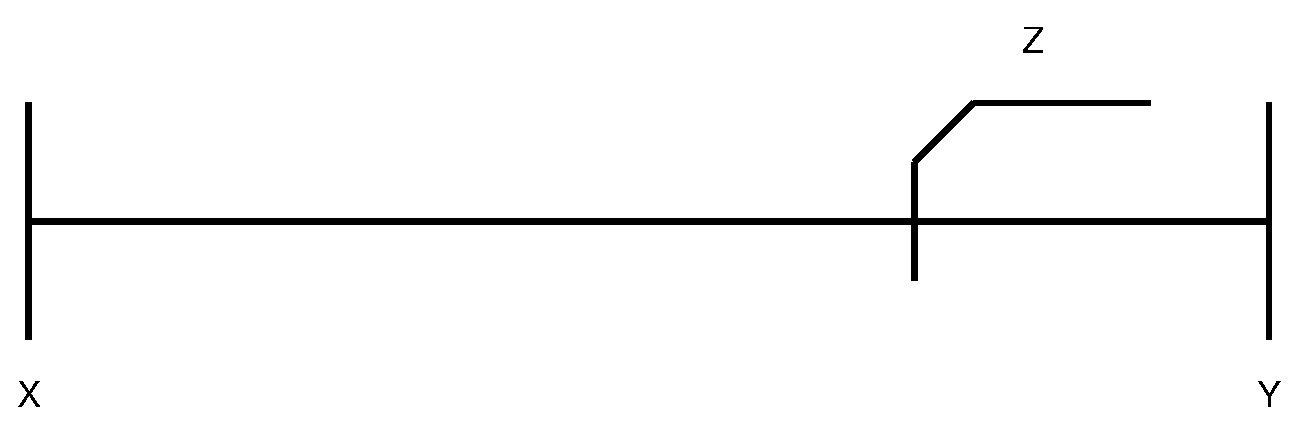
\includegraphics[scale=0.5]{\rootpath/worksheets/characteristics/figures/eval_example}
\caption{Example of characteristic evaluation scale}\label{fig:char_evel_example}
\end{figure}

In \bsref{fig:char_evel_example} \bscode{X} and \bscode{Y} represent the two extremes of the spectrum while \bscode{Z} along with its indicator represents where the model \bscode{Z} can be found upon the given spectrum. As an example \bscode{X} and \bscode{Y} could be implicit and explicit concurrency and \bscode{Z} could be the actor model. Using the placement of the example \bsref{fig:char_evel_example} would indicate that the actor model is mostly towards the explicit concurrency extreme. This is of course just an example placement.

Along with the placement of the selected model on the spectrum, a description of why the placement is as it is, will follow. When every model has been examined a summary and comparison of the selected models will be presented.\kasper{Reference chapter when created/done}
\worksheetend
